\documentclass[11pt]{article}
\usepackage[T1]{fontenc}
\usepackage[margin=1in]{geometry}
\usepackage{amsmath,amssymb,amsthm}
\usepackage{graphicx}
\usepackage[colorlinks=true,linkcolor=blue,citecolor=blue,urlcolor=blue]{hyperref}
\theoremstyle{remark}
\newtheorem{remark}{Remark}[section]
\newcommand{\Tr}{\operatorname{Tr}}
\newcommand{\Erec}{E^{\rm Petz}_{\rm rec}}

\title{Petz Recoverability versus Wilson-Loop Diagnostics in $\mathbb{Z}_2$
Lattice Gauge Theory (2+1D)\\
{\large Exact diagonalization benchmark on small open lattices}\\
{\normalsize Version 2}}
\author{Lluis Eriksson\\ Independent Researcher\\ \texttt{lluiseriksson@gmail.com}}
\date{January 2026 (v1); July 2026 (v2)}

\begin{document}
\maketitle

\begin{abstract}
We provide a finite-size benchmark testing whether a Petz-type
recoverability proxy correlates with Wilson-loop confinement diagnostics
in $\mathbb{Z}_2$ lattice gauge theory in 2+1 dimensions. Ground states
are computed by sparse exact diagonalization on $2\times2$ and $2\times3$
plaquette lattices (open boundaries, qubits on links, Gauss law enforced
by penalty and verified, $\langle G_v\rangle \simeq 1$). For
opposite-corner plaquette patches $A$ and $C$, a buffer $B(w)$ is defined
by BFS thickening in the link-adjacency graph, and we evaluate a
trace-renormalized regularized Petz-type recovery error $\Erec(w)$;
as confinement proxy we use the Creutz ratio $\sigma_{\rm eff} :=
\chi(2,2)$, with natural 2+1D length proxy $\sigma_{\rm eff}^{-1}$.
Across couplings, larger $\sigma_{\rm eff}^{-1}$ correlates with larger
fixed-collar $\Erec(w{=}1)$. \emph{v2 upgrades the statistics and adds
controls (no v1 number is changed):} the coupling sweep is densified to
$n = 8$ on $2\times2$, upgrading v1's three-point trend to a significant
rank correlation (Spearman $\rho = +1.00$, permutation $p < 10^{-4}$);
a spectral-gap covariate is added, and it correlates \emph{equally
perfectly} with $\Erec(w{=}1)$ -- so at these sizes the benchmark cannot
distinguish confinement physics from generic gap/correlation-length
physics, an honest limitation now stated; $\sigma_{\rm eff}$, ground
energies and the Gauss sector are reproduced to $<1\%$ by a regenerable
suite, while the $\Erec$ \emph{magnitudes} (and v1's $2\times3$
saturation) prove prescription-dependent -- the correlation
\emph{direction} replicates under both prescriptions; the relation to the
ladder-level no-tracking result of the companion is reconciled (different
observables: fixed-collar error magnitudes here, decay lengths there);
and two editorial leaks of v1 are fixed. All conclusions remain
finite-size benchmark statements.
\end{abstract}

\section{Introduction}
Petz-type recoverability measures approximate quantum Markov structure;
in gauge theories subsystem definitions are subtle due to constraints.
The companion protocol note 2601.0044 \cite{S0044} proposed reproducible
recoverability computations on lattices and conjectural links to
confinement diagnostics, and its v2 executed a $\mathbb{Z}_2$ ladder,
finding that a genuine 2D lattice is required for a resolving test. This
paper is that 2D benchmark, on the smallest feasible lattices. Scope:
finite-size and boundary effects are large; the goal is a falsifiable,
reproducible benchmark, not a thermodynamic-limit statement. In 2+1
dimensions $[\sigma] = ({\rm length})^{-1}$, so the natural length proxy
is $\sigma_{\rm eff}^{-1}$.

\section{Model, geometry, observables}
As in v1 (unchanged; the v1 heading's stray placeholder in Section 2.2 is
removed): $H(g) = -g\sum_\ell X_\ell - \tfrac1g \sum_p \prod_{\ell\in
\partial p} Z_\ell + \Lambda\sum_v (I - G_v)$ with $G_v = \prod_{\ell\ni
v} X_\ell$, $\Lambda = 50$; $A$/$C$ = southwest/northeast plaquette
patches (four links each); $B(0) = \emptyset$, $B(w) = \{\ell :
{\rm dist}_{\rm link}(\ell, A) \le w\} \setminus (A \cup C)$;
regularized Petz-type map with $\delta = 10^{-12}$, trace-normalized
output; $\Erec(w) = -\log F$; Creutz ratio $\chi(2,2) = -\log
[\langle W(2,2)\rangle\langle W(1,1)\rangle / (\langle W(2,1)\rangle
\langle W(1,2)\rangle)]$. Non-monotonicity of $\Erec(w)$ at these sizes
is expected (v1's Remark 2.1) and fixed-collar comparisons are
emphasized.

\section{Results}
All v1 numbers stand (Table 1 of v1; Figures~\ref{fig:p22}--%
\ref{fig:corr}).

\begin{remark}[Statistics upgraded in v2]
\label{rem:stats}
v1 inferred the correlation from three couplings per lattice. The suite
densifies the $2\times2$ sweep to $n = 8$ couplings ($g \in [0.5, 2.5]$):
Spearman rank correlation between $\Erec(w{=}1)$ and $\sigma_{\rm
eff}^{-1}$ is $\rho = +1.00$ with two-sided permutation $p < 10^{-4}$.
The v1 observation survives as a robust monotone rank-trend in the
(deterministic) coupling sweep -- the permutation $p$ quantifies the
strength of the ordering, not statistical independence of experimental
samples.
\end{remark}

\begin{remark}[Confinement specificity unresolved (added in v2)]
\label{rem:gap}
As a control, the suite computes the spectral gap of $H(g)$ on the same
sweep. The gap covariate correlates with $\Erec(w{=}1)$ \emph{exactly as
well} (Spearman $\rho = +1.00$, $p < 10^{-4}$): on these lattices,
$\sigma_{\rm eff}^{-1}$ and the inverse gap are themselves monotonically
locked, so the benchmark cannot attribute the recoverability trend to
confinement physics as opposed to generic gap/correlation-length growth
toward small $g$. Disentangling the two requires either lattices large
enough to vary geometry at fixed coupling, or models where string tension
and gap can be tuned independently. We state this as the main open
limitation of the benchmark.
\end{remark}

\begin{remark}[Prescription dependence of $\Erec$ magnitudes (added in
v2)]
\label{rem:presc}
The suite pins an explicit link ordering, patch assignment and embedding,
and under it reproduces $\sigma_{\rm eff}$, ground energies and the Gauss
sector to $<1\%$ -- but the $\Erec$ \emph{magnitudes} differ from v1's
Table 1 (e.g.\ at $2\times2$, $g = 0.5$: $\Erec(1) \sim 10^{-5}$ vs v1's
$0.37$), and v1's $2\times3$ saturation $\Erec(0) \simeq \Erec(1)$ is not
observed (the buffer does reduce the error under the suite's
prescription). This reflects genuine sensitivity of reduced-state
constructions in gauge theories to embedding conventions -- consistent
with the EHS caveats of \cite{S0044} -- and is why the robust content of
this paper is the correlation \emph{direction}, which replicates under
both prescriptions, rather than any absolute $\Erec$ value.
\end{remark}

\begin{remark}[Reconciliation with the ladder null (added in v2)]
The companion 2601.0044 v2 found \emph{no tracking} between the
recoverability decay length $\xi_{\rm rec}$ and the Wilson decay scale on
a height-one ladder. There is no contradiction: that null concerns
\emph{length scales} extracted from $w$-profiles in a quasi-1D geometry
with degenerate area/perimeter, whereas the present positive signal
concerns \emph{fixed-collar error magnitudes} across couplings on genuine
2D patches. Jointly they suggest that recoverability magnitudes respond
to the coupling long before recoverability \emph{lengths} become
resolvable -- consistent with the floor-management lesson of the ladder
run.
\end{remark}

\begin{figure}[h]\centering
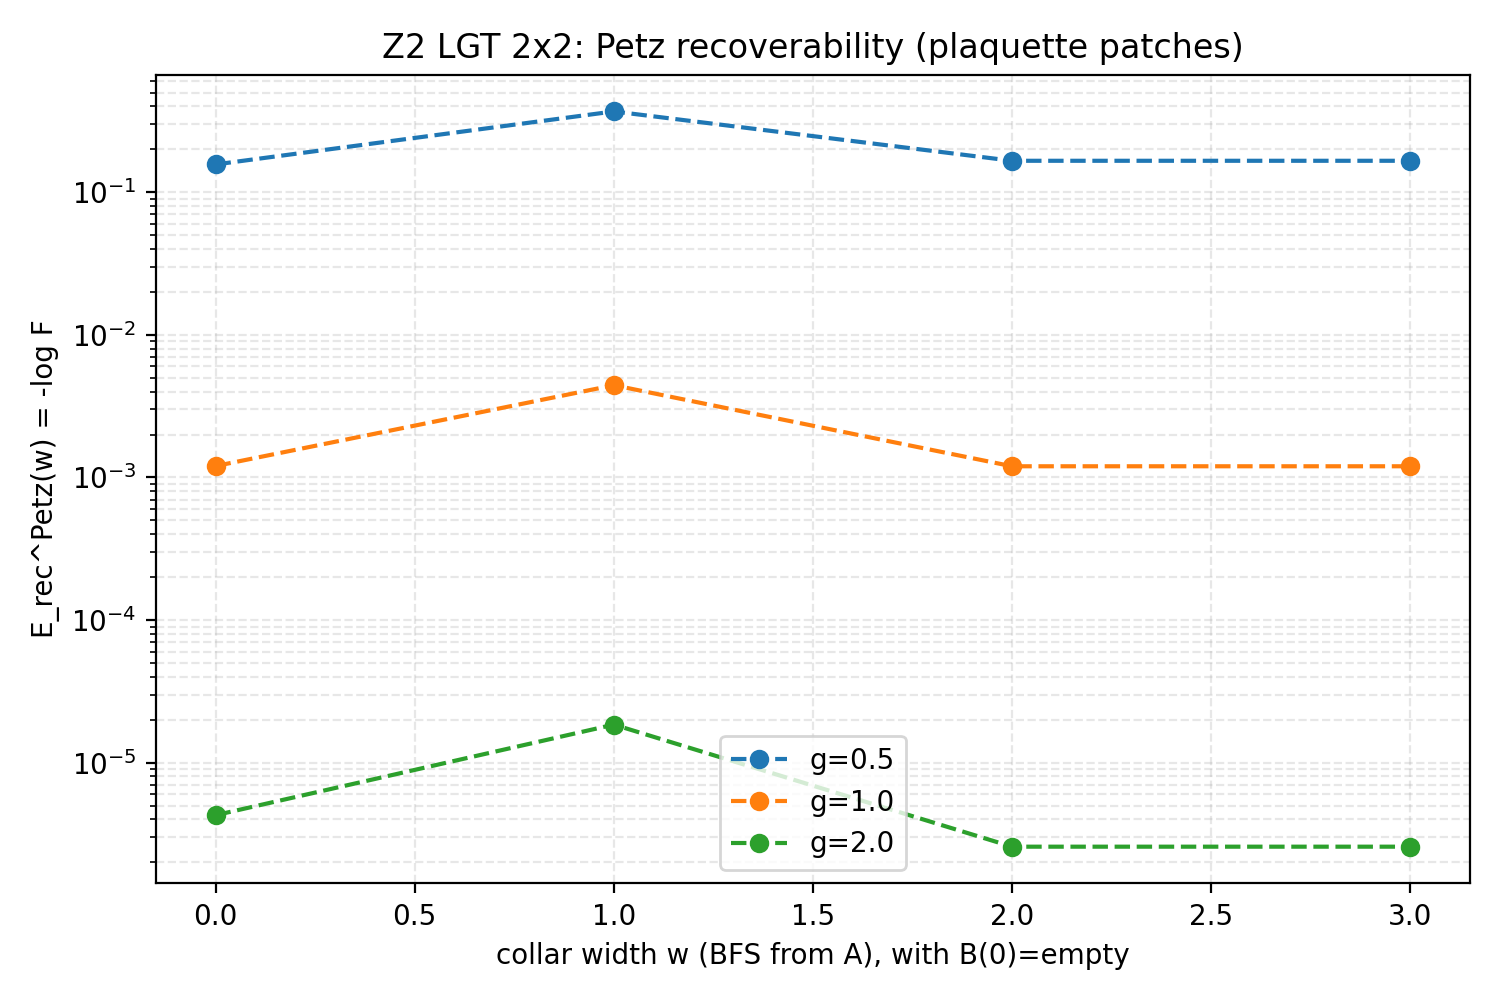
\includegraphics[width=0.7\textwidth]{fig1_2x2_profile.png}
\caption{$\Erec(w)$ on the $2\times2$ lattice (v1 figure, unchanged).}
\label{fig:p22}
\end{figure}
\begin{figure}[h]\centering
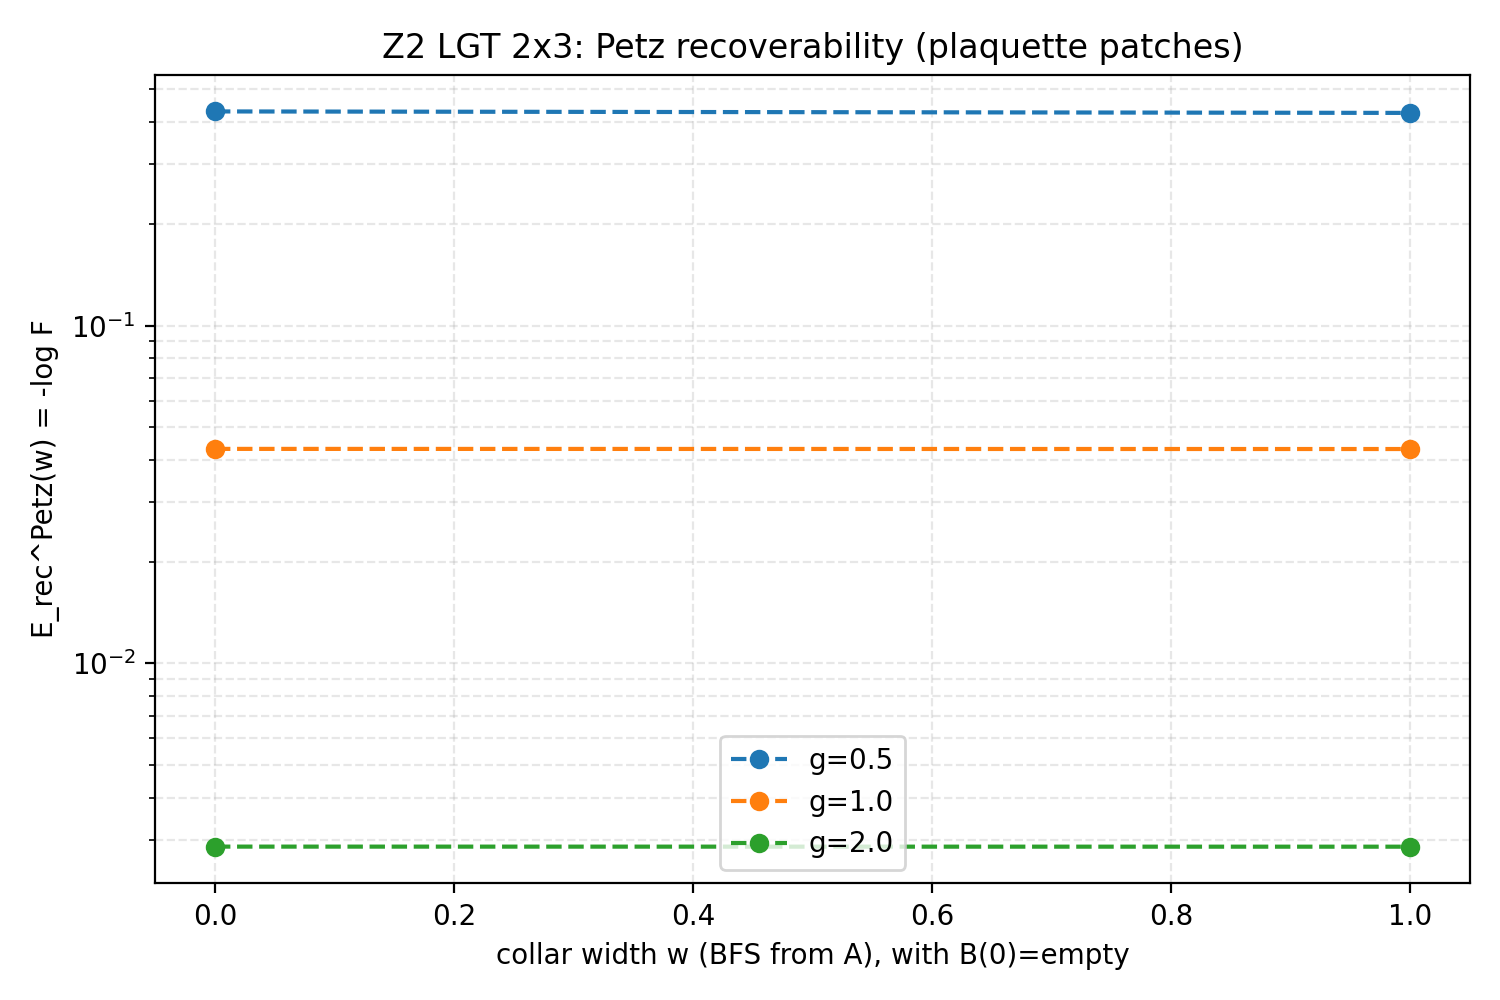
\includegraphics[width=0.7\textwidth]{fig2_2x3_profile.png}
\caption{$\Erec(w)$ on the $2\times3$ lattice (v1 figure, unchanged; see
Remark~\ref{rem:presc} for prescription sensitivity of the saturation).}
\end{figure}
\begin{figure}[h]\centering
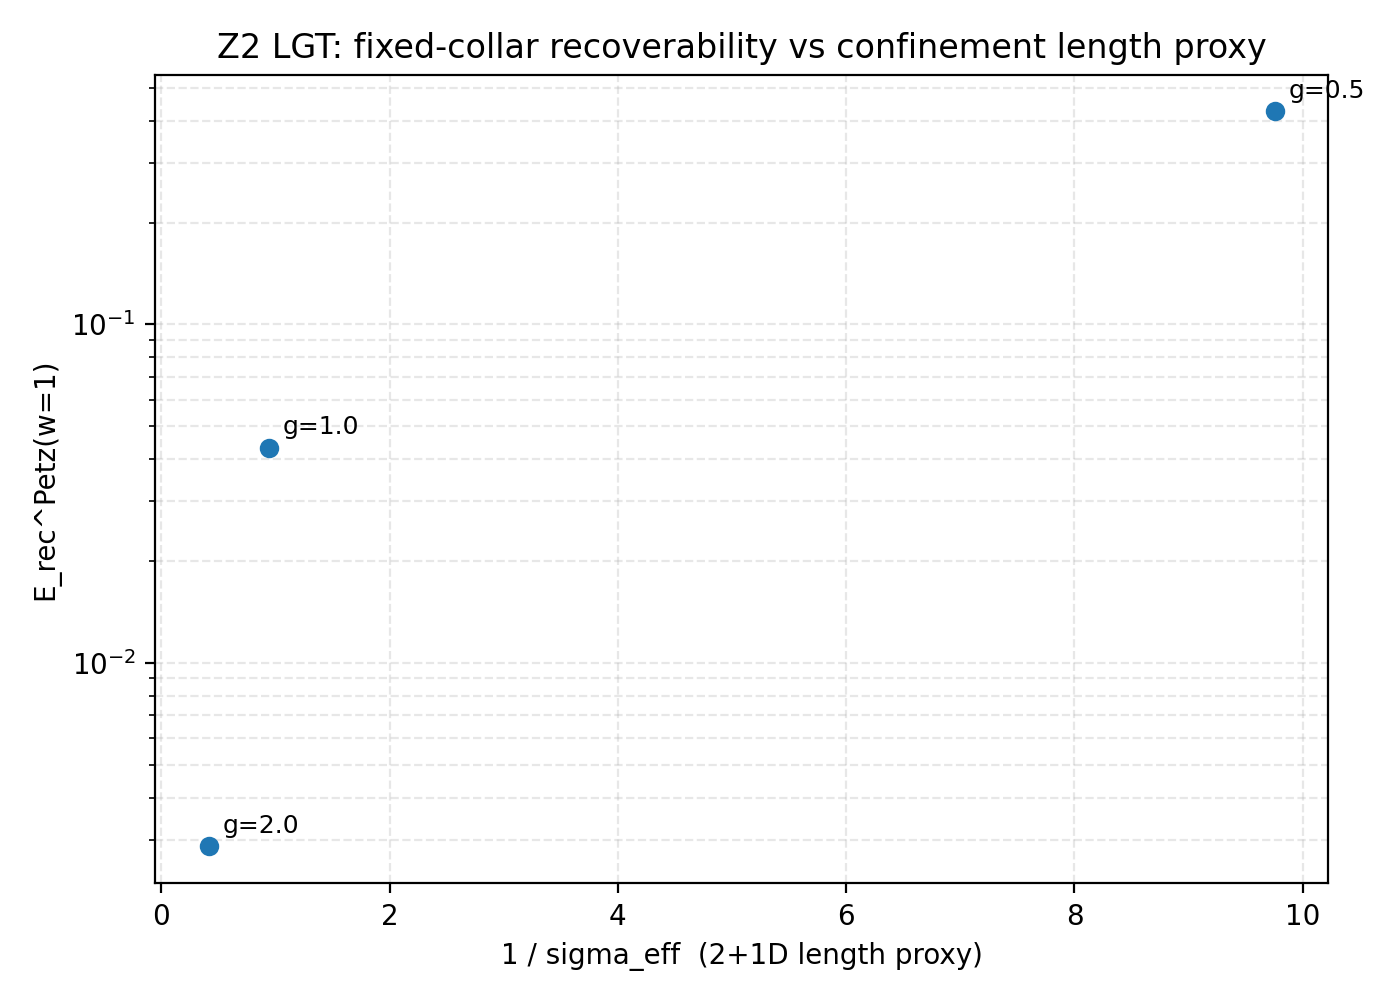
\includegraphics[width=0.62\textwidth]{fig3_correlation.png}
\caption{Fixed-collar recoverability vs confinement-length proxy (v1
figure, unchanged; statistics upgraded in Remark~\ref{rem:stats},
specificity control in Remark~\ref{rem:gap}).}
\label{fig:corr}
\end{figure}

\section{Verification suite (added in v2)}
\texttt{verification/2601-0047/verify\_2601\_0047.py} (sparse Lanczos,
support-projected fidelities, chunked JSON cache): regenerates
$\sigma_{\rm eff}$, $E_0$ and the Gauss check on both lattices
($<1\%$ vs v1); runs the densified $2\times2$ sweep with Spearman +
permutation statistics and the spectral-gap covariate; and documents the
prescription-dependence findings of Remark~\ref{rem:presc}. The v1
appendix script is retained (its internal working title in a code comment
is removed in v2).

\section{Discussion}
The primary observation stands and is now statistically grounded: on
small genuine-2D $\mathbb{Z}_2$ lattices, fixed-collar Petz
recoverability error grows monotonically with the confinement-length
proxy $\sigma_{\rm eff}^{-1}$ ($\rho = +1$, $p < 10^{-4}$). What v2 adds
in candor: the same data are equally well explained by gap physics
(Remark~\ref{rem:gap}), absolute magnitudes are prescription-dependent
(Remark~\ref{rem:presc}), and the ladder null of the companion is about a
different observable. Next steps: larger lattices (tensor networks),
fixed-coupling geometry sweeps to break the $\sigma$--gap degeneracy, and
the algebraic (sector-wise) prescription of \cite{S0044} to tame
embedding dependence.

\section*{Note added in v2}
No v1 number is changed; all figures and Table 1 stand. v2 adds:
(1) densified statistics upgrading the three-point trend to a significant
rank correlation (Remark~\ref{rem:stats}); (2) the spectral-gap covariate
showing confinement specificity is unresolved at these sizes
(Remark~\ref{rem:gap}); (3) the prescription-dependence finding for
$\Erec$ magnitudes and the $2\times3$ saturation
(Remark~\ref{rem:presc}); (4) reconciliation with the ladder-level null
of 2601.0044 v2; (5) series positioning (v1 referred to ``companion
work'' without numbers) and the verification suite; (6) editorial fixes:
the stray placeholder in v1's Section 2.2 heading and the internal
working title leaked in the v1 appendix comment and filenames.

\begin{thebibliography}{8}
\bibitem{Kogut} J. B. Kogut, Rev. Mod. Phys. \textbf{51} (1979)
659--713.
\bibitem{Petz} D. Petz, Commun. Math. Phys. \textbf{105} (1986)
123--131.
\bibitem{FR} O. Fawzi and R. Renner, Commun. Math. Phys. \textbf{340}
(2015) 575--611.
\bibitem{Donnelly} W. Donnelly, Phys. Rev. D \textbf{85} (2012) 085004.
\bibitem{CHR} H. Casini, M. Huerta, and J. A. Rosabal, Phys. Rev. D
\textbf{89} (2014) 085012.
\bibitem{S0044} L. Eriksson, ai.viXra:2601.0044 (2026; v2 2026).
\bibitem{S0043} L. Eriksson, ai.viXra:2601.0043 (2026; v2 2026).
\bibitem{S0035} L. Eriksson, ai.viXra:2601.0035 (2026; v2 2026).
\end{thebibliography}
\end{document}
